\documentclass{article}

% ready for submission
% \usepackage[nonatbib]{neurips_2025}


% to compile a preprint version, e.g., for submission to arXiv, add add the
% [preprint] option:
\usepackage[preprint, nonatbib]{neurips_2025}


% to compile a camera-ready version, add the [final] option, e.g.:
% \usepackage[final, nonatbib]{neurips_2025}


\usepackage[utf8]{inputenc} % allow utf-8 input
\usepackage[T1]{fontenc}    % use 8-bit T1 fonts
\usepackage{hyperref}       % hyperlinks
\usepackage{url}            % simple URL typesetting
\usepackage{booktabs}       % professional-quality tables
\usepackage{amsfonts}       % blackboard math symbols
\usepackage{nicefrac}       % compact symbols for 1/2, etc.
\usepackage{microtype}      % microtypography
\usepackage{xcolor}         % colors

% ---------------------------------------------------------------------------- %
% TODO: CUSTOM PACKAGES
% -----------------------------------------------------------------------------
%  Encoding & fonts
% -----------------------------------------------------------------------------
\usepackage[utf8]{inputenc}  % allow UTF‑8 input
\usepackage[T1]{fontenc}     % 8‑bit T1 fonts

% -----------------------------------------------------------------------------
%  Maths & symbols
% -----------------------------------------------------------------------------
\usepackage{amsmath,amssymb,amsfonts}
\usepackage{mathtools}
\usepackage{bm}              % bold maths symbols

% -----------------------------------------------------------------------------
%  Graphics & floats
% -----------------------------------------------------------------------------
\usepackage{graphicx}
\usepackage{subcaption}
\graphicspath{{figures/}}    % all figures live here
\usepackage{booktabs}        % professional tables
\usepackage{siunitx}
\sisetup{detect-all}
\usepackage{paralist}

% -----------------------------------------------------------------------------
%  Microtype & formatting helpers
% -----------------------------------------------------------------------------
\usepackage{microtype}
\usepackage{nicefrac}        % compact 1/2 etc.
\usepackage{xcolor}

% -----------------------------------------------------------------------------
%  Bibliography (biblatex, IEEE style)
% -----------------------------------------------------------------------------
\usepackage[
backend=biber,
style=ieee,
sorting=nyt,
giveninits=true,
maxbibnames=99,
doi=false,isbn=false,url=false
]{biblatex}
\addbibresource{ref.bib}

% -----------------------------------------------------------------------------
%  Clever references – after hyperref!
% -----------------------------------------------------------------------------
\usepackage{hyperref}
\usepackage[capitalise]{cleveref}

% -----------------------------------------------------------------------------
%  Algorithms (optional – comment out if unused)
% -----------------------------------------------------------------------------
\usepackage[ruled,vlined]{algorithm2e}
\SetKwInOut{Input}{Input}
\SetKwInOut{Output}{Output}

% -----------------------------------------------------------------------------
%  Custom macros
% -----------------------------------------------------------------------------
\newcommand{\ours}{\textsc{ViT‑Reg}\xspace}
\newcommand{\RegTok}{\texttt{[REG]}\xspace}
\newcommand{\nreg}{N}
% Natbib‑style aliases for biblatex users who prefer natbib commands
\newcommand{\citet}{\textcite}
\newcommand{\citep}{\parencite}
\newcommand{\todo}[1]{\textcolor{red}{TODO: #1}}
\newcommand{\ntok}{T}

\crefname{section}{§}{§§}
\crefname{table}{Table}{Tables}
\crefname{figure}{Fig.}{Figs.}
% ---------------------------------------------------------------------------- %

\title{A Study on ``Vision Transformers Need Registers''}

\author{%
  Juntang~Wang\thanks{Personal webpage: \url{https://tang.qqgjyx.com}} \\
  Duke Kunshan University\\
  Kunshan, Jiangsu Province, China \\
  \texttt{jw853@duke.edu} \\
  \And
  Hao~Wu \\
  Sichuan University \\
  Chengdu, Sichuan Province, China \\
  \texttt{hwu@scu.edu.cn}
}

\begin{document}


\maketitle



% ---------------------------------------------------------------------------- %
%  ABSTRACT – 200 words max
% ---------------------------------------------------------------------------- %
\begin{abstract}
    Learning generic features for real-world data has long been a central goal in machine learning.
    Leveraging submodules from supervised or self-supervised models as feature extractors has attracted increasing attention in recent years.
    Among these, Vision Transformers (ViTs) have shown strong performance—but occasionally produce \emph{high‑norm outlier tokens} in low‑information image regions, degrading downstream dense‑prediction tasks.
    To mitigate this, Darcet~\emph{et~al.} propose register tokens—learnable placeholders discarded at output—as a lightweight remedy. 
    In this report, we reproduce their key findings, port the method to several new real‑world benchmarks, and introduce an \emph{adaptive register allocator} that learns the pseudo‑optimal number of registers online.
  % Code is released at \url{https://github.com/your‑lab/vit‑registers‑plus}.
\end{abstract}



% ---------------------------------------------------------------------------- %
%  INTRODUCTION
% ---------------------------------------------------------------------------- %
\section{Introduction}
\label{sec:intro}
Embedding real-world data into general-purpose features has long been a central goal in machine learning.
Classical methods such as PCA~\citep{jolliffePrincipalComponentAnalysis1986}, t-SNE~\citep{van2008visualizing}, and SIFT~\citep{loweDistinctiveImageFeatures2004} rely on strong handcrafted assumptions and were widely used prior to the rise of deep learning. 
The pursuit of general-purpose features remains relevant today, largely because labeled data is expensive—either due to scale or the need for domain expertise (\emph{e.g.}, medical imaging or language translation).

Under the transfer‑learning paradigm, a common strategy is to pretrain a model on a data‑rich task and later reuse part of that model as a frozen feature extractor for downstream problems.
Beyond conventional supervised pretraining, self‑supervised methods—especially Vision Transformers (ViTs)—have gained prominence for two reasons: (i) they achieve strong downstream accuracy and (ii) some of them, such as DINO~\citep{caronEmergingPropertiesSelfsupervised2021}, exhibit the striking ability to delineate objects without any labels, as illustrated in~\cref{fig:attn6}.
Recent work shows that such self‑supervised ViTs can be “pretrained once, reused everywhere,” providing generic visual features that rival those from fully supervised counterparts~\citep{caronEmergingPropertiesSelfsupervised2021, oquabDINOv2LearningRobust2024}.

\begin{figure}[h]
    \centering
    \includegraphics[width=\textwidth]{figures/attn6.png}
    \caption{Attention maps from the \texttt{[CLS]} query produced by the last attention layer~\citep{caronEmergingPropertiesSelfsupervised2021}.}
    \label{fig:attn6}
\end{figure}

Leveraging DINO’s patch‑level features, object‑discovery algorithms such as LOST~\citep{simeoniLocalizingObjectsSelfsupervised2021} can localize objects without supervision.
DINOv2~\citep{oquabDINOv2LearningRobust2024}—a follow‑up trained to excel at dense prediction—indeed yields strong frozen‑backbone results on monocular depth and semantic segmentation, yet performs surprisingly poorly when paired with LOST~\citep{darcetVisionTransformersNeed2024}.
This discrepancy suggests that DINOv2’s representations differ qualitatively from DINO’s and motivates a closer inspection of ViT feature maps.

\citet{darcetVisionTransformersNeed2024} traced this failure to \emph{artifacts} present in most ViTs—including DINOv2, but absent from DINO. 
These artifacts appear as patch tokens whose $\ell_2$‑norm is abnormally large yet encode little local information (see~\cref{fig:allvits}). 
Such outliers corrupt methods like LOST, which assume smooth, semantically meaningful feature maps. 
Similar artifacts also surface in several supervised Vision Transformers, underscoring that DINO is the exception rather than the rule.

\begin{figure}[t]
    \centering
    {\footnotesize
    \setlength{\tabcolsep}{2.5pt} %
    \renewcommand{\arraystretch}{0.4} %
    \begin{tabular}{c cc cc cc }
      \vspace{0.2em}
      Input & DeiT-III-B & DeiT-III-L & OpenCLIP-B & OpenCLIP-L & DINO-B & DINOv2-g \\
      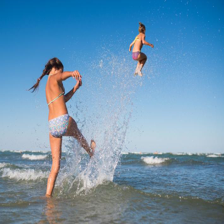
\includegraphics[width=0.13\textwidth]{resources/230914_1202_fig2_vizs_various_models/109_orig.png} &
      
\includegraphics[width=0.13\textwidth]{resources/230914_1202_fig2_vizs_various_models/deit3_base_patch16_224.fb_in22k_ft_in1k_109_lastattmap.png} &
      
\includegraphics[width=0.13\textwidth]{resources/230914_1202_fig2_vizs_various_models/deit3_large_patch16_224.fb_in22k_ft_in1k_109_lastattmap.png} &
      
\includegraphics[width=0.13\textwidth]{resources/230914_1202_fig2_vizs_various_models/vit_base_patch16_clip_224.laion2b_109_lastattmap.png} &
      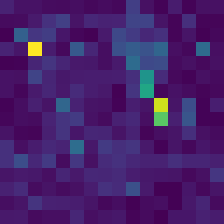
\includegraphics[width=0.13\textwidth]{resources/230914_1202_fig2_vizs_various_models/vit_large_patch14_clip_224.laion2b_109_lastattmap.png} &
      
\includegraphics[width=0.13\textwidth]{resources/230914_1202_fig2_vizs_various_models/vit_base_patch16_224.dino_109_lastattmap.png} &
      
\includegraphics[width=0.13\textwidth]{resources/230914_1202_fig2_vizs_various_models/vit_giant_patch14_dinov2.lvd142m_109_lastattmap.png}
      \\
      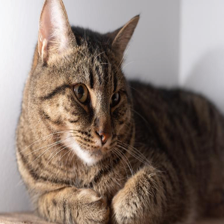
\includegraphics[width=0.13\textwidth]{resources/230914_1202_fig2_vizs_various_models/1500_orig.png} &
      
\includegraphics[width=0.13\textwidth]{resources/230914_1202_fig2_vizs_various_models/deit3_base_patch16_224.fb_in22k_ft_in1k_1500_lastattmap.png} &
      
\includegraphics[width=0.13\textwidth]{resources/230914_1202_fig2_vizs_various_models/deit3_large_patch16_224.fb_in22k_ft_in1k_1500_lastattmap.png} &
      
\includegraphics[width=0.13\textwidth]{resources/230914_1202_fig2_vizs_various_models/vit_base_patch16_clip_224.laion2b_1500_lastattmap.png} &
      
\includegraphics[width=0.13\textwidth]{resources/230914_1202_fig2_vizs_various_models/vit_large_patch14_clip_224.laion2b_1500_lastattmap.png} &
      
\includegraphics[width=0.13\textwidth]{resources/230914_1202_fig2_vizs_various_models/vit_base_patch16_224.dino_1500_lastattmap.png} &
      
\includegraphics[width=0.13\textwidth]{resources/230914_1202_fig2_vizs_various_models/vit_giant_patch14_dinov2.lvd142m_1500_lastattmap.png}
      \\
      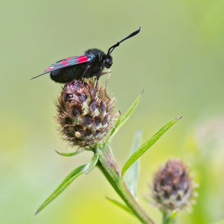
\includegraphics[width=0.13\textwidth]{resources/230914_1202_fig2_vizs_various_models/85_orig.png} &
      
\includegraphics[width=0.13\textwidth]{resources/230914_1202_fig2_vizs_various_models/deit3_base_patch16_224.fb_in22k_ft_in1k_85_lastattmap.png} &
      
\includegraphics[width=0.13\textwidth]{resources/230914_1202_fig2_vizs_various_models/deit3_large_patch16_224.fb_in22k_ft_in1k_85_lastattmap.png} &
      
\includegraphics[width=0.13\textwidth]{resources/230914_1202_fig2_vizs_various_models/vit_base_patch16_clip_224.laion2b_85_lastattmap.png} &
      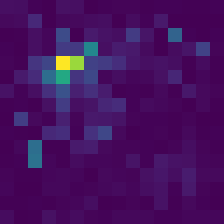
\includegraphics[width=0.13\textwidth]{resources/230914_1202_fig2_vizs_various_models/vit_large_patch14_clip_224.laion2b_85_lastattmap.png} &
      
\includegraphics[width=0.13\textwidth]{resources/230914_1202_fig2_vizs_various_models/vit_base_patch16_224.dino_85_lastattmap.png} &
      
\includegraphics[width=0.13\textwidth]{resources/230914_1202_fig2_vizs_various_models/vit_giant_patch14_dinov2.lvd142m_85_lastattmap.png}
      \\
      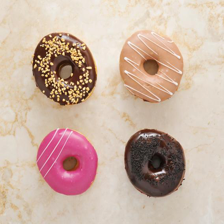
\includegraphics[width=0.13\textwidth]{resources/230914_1202_fig2_vizs_various_models/1753_orig.png} &
      
\includegraphics[width=0.13\textwidth]{resources/230914_1202_fig2_vizs_various_models/deit3_base_patch16_224.fb_in22k_ft_in1k_1753_lastattmap.png} &
      
\includegraphics[width=0.13\textwidth]{resources/230914_1202_fig2_vizs_various_models/deit3_large_patch16_224.fb_in22k_ft_in1k_1753_lastattmap.png} &
      
\includegraphics[width=0.13\textwidth]{resources/230914_1202_fig2_vizs_various_models/vit_base_patch16_clip_224.laion2b_1753_lastattmap.png} &
      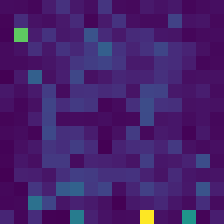
\includegraphics[width=0.13\textwidth]{resources/230914_1202_fig2_vizs_various_models/vit_large_patch14_clip_224.laion2b_1753_lastattmap.png} &
      
\includegraphics[width=0.13\textwidth]{resources/230914_1202_fig2_vizs_various_models/vit_base_patch16_224.dino_1753_lastattmap.png} &
      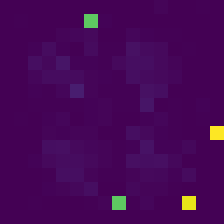
\includegraphics[width=0.13\textwidth]{resources/230914_1202_fig2_vizs_various_models/vit_giant_patch14_dinov2.lvd142m_1753_lastattmap.png}
      \\
    \end{tabular}
    }
    \caption{
      We consider ViTs trained with label supervision (DeiT-III), text-supervision (OpenCLIP) or self-supervision (DINO and DINOv2).
      \emph{All models but DINO} exhibit peaky outlier values in the attention maps~\cite{darcetVisionTransformersNeed2024}.
    }  
    \label{fig:allvits}
\end{figure}

As a remedy and inspired by~\citet{bulatovRecurrentMemoryTransformer2022}, \citet{darcetVisionTransformersNeed2024} prepend a small set of learnable register tokens (\RegTok) to the input sequence; these tokens absorb global context and are dropped before features are fed to downstream heads. 
Empirically, this simple change suppresses artifacts and consistently restores—sometimes even improves—performance on tasks sensitive to feature‑map quality.

Beyond replication, our contributions would include:

\paragraph{Cross‑domain extension.}
Beyond classic CV benchmarks, we extend the register‑token idea to sequence‑modeling and tabular settings, and uncover analogous artifacts in those modalities.

\paragraph{New observations.}
During this exploration we identify two phenomena:  
\begin{enumerate}
    \item Certain \RegTok tokens behave similarly to components discovered by our
          Multi‑Resolution Graph‑based Clustering method (GraMixC; see Appendix~\ref{sec:gmc}).
    \item Registers acquire a stable, \emph{position‑dependent} ordering—appending them
          after patch tokens yields one specialization order ($\text{reg}_1\!\rightarrow\!\text{reg}_r$),
          prepending reverses it, and scrambling positional encoding destroys the effect and
          degrades performance.
\end{enumerate}

\paragraph{Adaptive allocation.}
Motivated by these findings, we introduce an \emph{adaptive register allocator} that learns a pseudo‑optimal number of registers online; across diverse tasks it converges to the same “best” register count, matching or exceeding the performance of fixed‑register baselines.



% ---------------------------------------------------------------------------- %
% Related work
% ---------------------------------------------------------------------------- %
\section{Related Work}
\label{sec:related}

\paragraph{Universal representation learning.}
The idea of “learn once, transfer everywhere” began with distributed word embeddings (\emph{e.g.}, word2vec, GloVe) and BERT‑style masked‑language pre‑training \citep{devlinBERTPretrainingDeep2019}.
Comparable trends followed in speech, with wav2vec 2.0 \citep{baevskiWav2vec20Framework2020a}, and in vision, where ImageNet‑pretrained CNNs were the standard backbone for nearly a decade \citep{krizhevskyImageNetClassificationDeep2012}.  
Across modalities the economic rationale is the same: labels are scarce, raw data abundant.

\paragraph{Visual backbones—supervised and self‑supervised.}
Self‑supervised objectives such as SimCLR, MoCo, BYOL, and MAE demonstrated that high‑capacity encoders can be trained without labels \citep{chenSimpleFrameworkContrastive2020,heMomentumContrastUnsupervised,grillBootstrapYourOwn2020,heMaskedAutoencodersAre2022}.  
When these ideas met Vision Transformers, \textbf{DINO} (\emph{Distillation with No Labels}) \citep{caronEmergingPropertiesSelfsupervised2021} produced attention maps that align with object masks; its successor \textbf{DINOv2} \citep{oquabDINOv2LearningRobust2024} pushed dense‑prediction scores higher but introduced the high‑norm outliers that motivate our study.

\vspace{0.3em}\noindent
\textbf{Baselines evaluated in this study.}  
Because our remedy is an architectural drop‑in, we can attach it to any training procedure.  
To span the supervision spectrum we adopt three state‑of‑the‑art ViT checkpoints trained on distinct data sources:

\begin{itemize}
  \item \textbf{DeiT‑III} \citep{touvronDeiTIIIRevenge2022} — a label‑supervised recipe that trains a ViT‑B/16 on ImageNet‑22k \citep{dengImageNetLargescaleHierarchical2009}.
        It is simple, uses the vanilla ViT backbone, achieves strong classification accuracy, and is easy to reproduce and modify.  
        We use the official ImageNet‑22k, ViT‑B configuration.\footnote{\url{https://github.com/facebookresearch/deit}}
  \item \textbf{OpenCLIP} \citep{ilharco_gabriel_2021_5143773} — an open‑source text–image contrastive model that aligns ViT‑B/16 with captions drawn from a licensed Shutterstock subset and LAION‑2B \citep{schuhmannLAION5BOpenLargescale2022}.
        It represents the text‑supervised regime and is likewise straightforward to reproduce and extend.\footnote{\url{https://github.com/mlfoundations/open_clip}}
  \item \textbf{DINOv2} \citep{oquabDINOv2LearningRobust2024} — a self‑supervised ViT‑L/16 trained on ImageNet‑22k; it delivers state‑of‑the‑art dense‑prediction scores yet suffers from high‑norm outlier artifacts that motivate our work.
        All experiments follow the public ViT‑L recipe.\footnote{\url{https://github.com/facebookresearch/dinov2}}
\end{itemize}

\paragraph{Auxiliary and memory tokens in Transformers.}
Special tokens have long served as delimiters (\texttt{[SEP]} in BERT), classification heads (\texttt{[CLS]}), or latent bottlenecks (Perceiver‑IO) \citep{devlinBERTPretrainingDeep2019,jaeglePerceiverIOGeneral2021}.  
In language, Transformer‑XL and RMT keep recurrent memory tokens \citep{bulatovRecurrentMemoryTransformer2022}; in vision, TokenLearner and DynamicViT drop low‑saliency tokens to save FLOPs \citep{ryooTokenLearnerAdaptiveSpacetime2021,raoDynamicViTEfficientVision2021}.  
Register tokens \citep{darcetVisionTransformersNeed2024} flip this logic by \emph{adding} a few learnable slots that absorb global context and are discarded before prediction.

\paragraph{Artifact analysis in ViTs.}
Token‑norm statistics have inspired pruning schemes such as PatchDropout and EvoViT \citep{liuPatchDropoutEconomizingVision2023,xuEvoViTSlowfastToken2022}.  
\citet{darcetVisionTransformersNeed2024} revealed the opposite pathology: excessively large‑norm tokens concentrate in low‑information regions and harm dense tasks.  
A recent reproducibility study \citep{ReproducibilityStudyVision2025} confirms that register tokens or norm regularisation mitigates these artifacts; our experiments extend this finding to sequence and tabular modalities.

\paragraph{Transformers beyond vision.}
Self‑attention has become a universal building block:  
TabTransformer and SAINT treat table columns as token sequences \citep{huangTabTransformerTabularData2020,somepalliSAINTImprovedNeural2021};  
Enformer brings long‑range attention to genomics \citep{avsecEffectiveGeneExpression2021};  
AST and wav2vec 2.0 model audio \citep{gongASTAudioSpectrogram2021,baevskiWav2vec20Framework2020a};  
and Perceiver‑IO offers a modality‑agnostic latent array \citep{jaeglePerceiverIOGeneral2021}.  
Prior work has not examined whether these non‑vision Transformers exhibit the \emph{high‑norm outlier} pathology.  
We are the first to \todo{uncover such artifacts}—and to show the benefits of register tokens in sequence and tabular benchmarks.

\paragraph{Adaptive resource allocation.}
Dynamic architectures such as LayerScale, DeepMoE, and early‑exit Transformers learn to allocate depth or width per input \citep{touvronGoingDeeperImage2021, wangDeepMixtureExperts2019}.  
Our \emph{adaptive register allocator} follows this line: rather than fixing the number of registers, it predicts an input‑specific count and converges to a consistent optimum across tasks.

\smallskip
In summary, our study links generic representation learning, auxiliary‑token design, and Transformer interpretability.  
By extending register tokens across modalities and introducing an adaptive allocator, we broaden this line of research beyond vision alone.



% ---------------------------------------------------------------------------- %
% Methodology
% ---------------------------------------------------------------------------- %
\section{Methodology}
\label{sec:method}



\subsection{Preliminaries — Detecting and Explaining ViT Artifacts}
\label{sec:prelim}

Modern vision transformers occasionally produce a handful of \emph{patch tokens} whose $\ell_2$‑norm is \emph{orders of magnitude} larger than the norm of their neighbours.  
\citet{darcetVisionTransformersNeed2024} coined these tokens \emph{artifacts} and argued that they are the root cause of DINOv2’s failure on object‑discovery tasks.
Before we revisit their remedy, we replicate and systematise the empirical evidence behind this claim.

\paragraph{One‑line detector.}
For every output token $z_i\!\in\!\mathbb R^{d}$ we label it an artifact whenever 
\begin{equation}
\|z_i\|_{2}>\tau, \quad \tau=150.
\end{equation}
Where $\tau$ is a customized threshold, which we set to $150$ following the original study. \cref{fig:norms_hist} reproduces the bimodal norm histogram originally reported by \citet{darcetVisionTransformersNeed2024}:
DINOv2 (ViT‑g/14) exhibits a distinct heavy tail, whereas its predecessor DINO (ViT‑B/16) does not.
Across ImageNet‑val $2.37\,\%$ of DINOv2 tokens cross the $\tau$, large enough to hurt dense prediction.

\begin{figure}[t]
  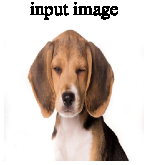
\includegraphics{resources/figure_3_1.pdf}
  
\includegraphics{resources/figure_3_2.pdf}
  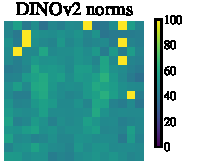
\includegraphics{resources/figure_3_3.pdf}
  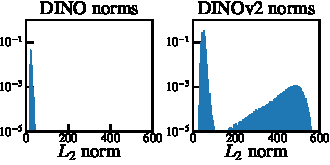
\includegraphics{resources/figure_3_4.pdf}
  \caption{
    Norm histograms for DINO (ViT-B/16) vs.\ DINOv2 (ViT-g/14). 
    The latter exhibits a distinct high-norm tail ($>$150) that comprises 2.37 \% of tokens, which is not observed in DINO~\citep{darcetVisionTransformersNeed2024}.}
  \label{fig:norms_hist}
\end{figure}

\paragraph{When and where do artifacts emerge?}
Using the public DINOv2 checkpoints we trace the phenomenon through training and scale (\cref{fig:factors_choice}):
(i) artifacts materialise around the middle of the 40‑layer ViT‑g and remain prominent to the output,
(ii) they appear after roughly the first third of pre‑training, and
(iii) they afflict \emph{only} the three largest model families (Large, Huge, Giant).
In other words, the behaviour is \emph{capacity‑dependent}; smaller ViTs such as DINO‑B are immune.

\begin{figure}[t]
  \centering
  \subcaptionbox{Norms along layers.\label{fig:norm_hist_by_layer}}{
    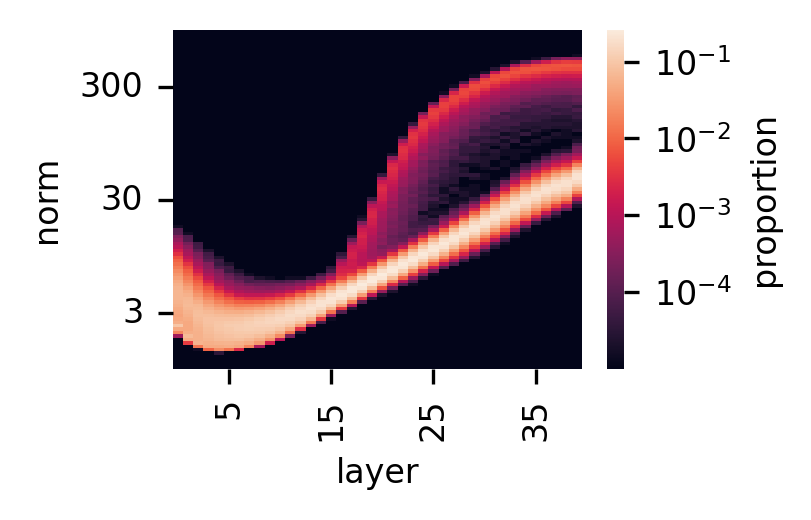
\includegraphics[width=0.31\linewidth]{resources/230802_norm_histogram_by_layer.png}
  }
  \subcaptionbox{Norms along iterations.\label{fig:norm_hist_by_iter}}{
    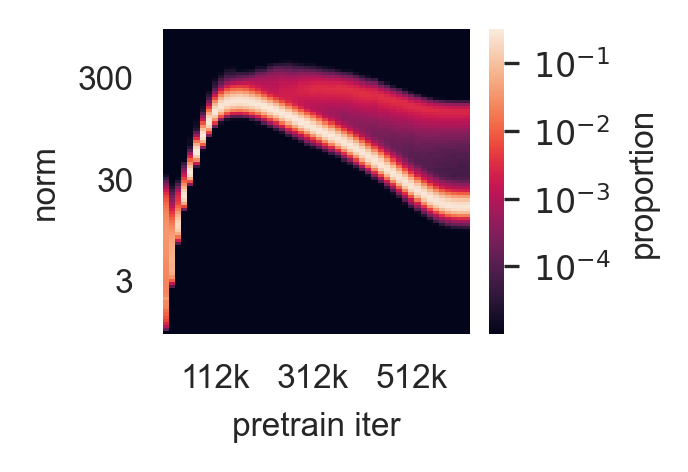
\includegraphics[width=0.31\linewidth]{resources/norm_distrib_vs_pretrain_iter.png}
  }
  \subcaptionbox{Norms across model size.\label{fig:norm_hist_by_model}}{
    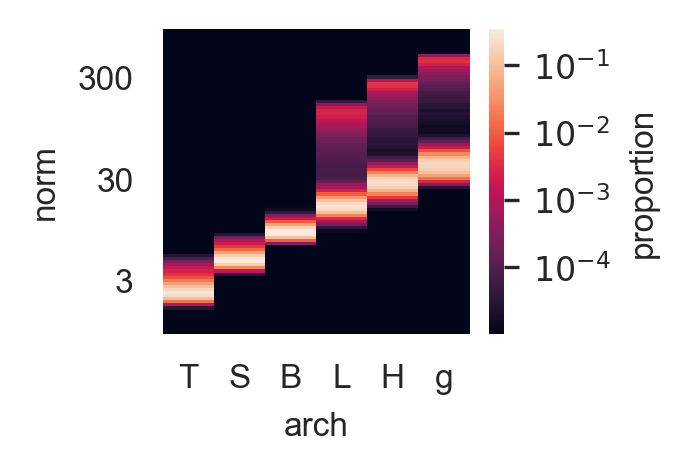
\includegraphics[width=0.31\linewidth]{resources/norm_distrib_vs_model_size.png}
  }
  \caption{
    Illustration of token norms in the 40-layer DINOv2 ViT-g model.
    \textbf{(a)}: Norms distribution along layers.
    \textbf{(b)}: Norms distribution along training iterations.
    \textbf{(c)}: Norms distribution for different model sizes. 
    Artifacts emerge as number of layers, training iterations, and model size increase~\citep{darcetVisionTransformersNeed2024}.}
  \label{fig:factors_choice}
\end{figure}

\paragraph{Spatial footprint: redundant patches.}
Plotting cosine similarity between each artifact and its four nearest patches (\cref{fig:outlier_cos_sims}) reveals that artifacts sit almost exclusively in background regions whose raw pixels are highly redundant.
Qualitatively, they coincide with sky, grass, whiteboards—areas a recognition model could trivially compress.
This also hinder the following local and global probes.

\begin{figure}[tb]
  \centering
  \subcaptionbox{Cosine similarity to neighbors.\label{fig:outlier_cos_sims}}{
    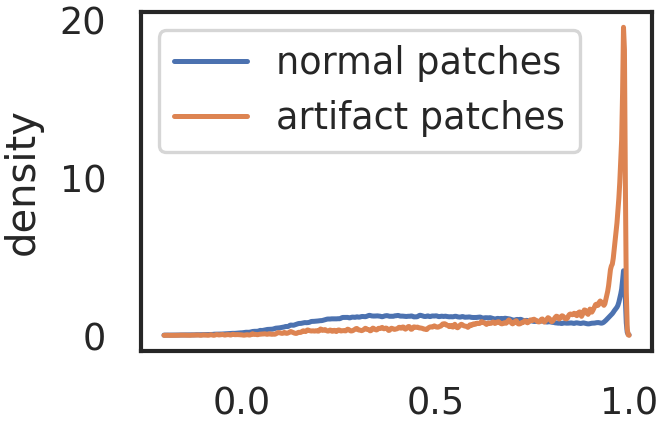
\includegraphics[width=0.3\linewidth]{resources/230802_kde_cossim_neighbors_2.png}
  }
  \hfill
  \subcaptionbox{Linear probing for local information.\label{tab:logreg_weird_patches_local}}{
    \begin{tabular}{@{} l c cc c c @{}}
      \toprule
              && \multicolumn{2}{c}{position prediction} && reconstruction\\
      \cmidrule{3-4} \cmidrule{6-6}
              && top-1 acc      & avg. distance $\downarrow$ && L2 error $\downarrow$\\
      \midrule
      normal  && \textbf{41.7}  & \textbf{0.79} && \textbf{18.38} \\
      outlier && 22.8           & 5.09          && 25.23 \\
      \bottomrule
    \end{tabular}
  }
  \caption{Artifacts sit in redundant patches and contain little local signal \citep{darcetVisionTransformersNeed2024}.}
\end{figure}

\paragraph{What information do artifacts encode?}
We probe the embeddings with two contrastive studies.
\begin{enumerate}
  \item \textbf{Local probes.} 
    A linear head trained to
    (a) predict patch position or 
    (b) reconstruct the RGB pixels performs significantly better on normal tokens than on artifacts (\cref{tab:logreg_weird_patches_local}).
    Metrics are chosen to be top-1 accuracy, average distance, and L2 error, in complete agreement with the original study.
    A conclusion is then made that artifacts \emph{discard local detail}.
  \item \textbf{Global probes.} 
    Conversely, randomly picking a single token to represent the whole image and training a logistic‑regression classifier, artifacts yield rival but comparable performance with the global \texttt{[CLS]} embedding and beat normal tokens on \emph{all} 14 benchmarks (\cref{tab:logreg_weird_patches_image_classif}).
    A conclusion is then made that artifacts \emph{accumulate global context}.
\end{enumerate}

\begin{table}[t]
  \centering
  \caption{Single‑token linear probes with ViT‑g features~\citep{darcetVisionTransformersNeed2024}.  
           Artifacts outperform normal patches and approach \texttt{[CLS]} on global tasks.}
  \label{tab:logreg_weird_patches_image_classif}
  \vspace{0.2em}
  \resizebox{\textwidth}{!}{%
  \begin{tabular}{@{}lcccccccccccccc@{}}
    \toprule
    & IN1k & P205 & Airc. & CF10 & CF100 & CUB & Cal101 & Cars & DTD & Flow. & Food & Pets & SUN & VOC \\
    \midrule
    \texttt{[CLS]} & \textbf{86.0} & \textbf{66.4} & \textbf{87.3} & \textbf{99.4} & \textbf{94.5} & \textbf{91.3} & 96.9 & \textbf{91.5} & \textbf{85.2} & \textbf{99.7} & \textbf{94.7} & \textbf{96.9} & \textbf{78.6} & 89.1 \\
    Normal         & 65.8 & 53.1 & 17.1 & 97.1 & 81.3 & 18.6 & 73.2 & 10.8 & 63.1 & 59.5 & 74.2 & 47.8 & 37.7 & 70.8 \\
    Artifact       & 69.0 & 55.1 & 79.1 & 99.3 & 93.7 & 84.9 & \textbf{97.6} & 85.2 & 84.9 & 99.6 & 93.5 & 94.1 & 78.5 & \textbf{89.7} \\
    \bottomrule
  \end{tabular}}
  \vspace{-1em}
\end{table}

\paragraph{Mechanistic hypothesis.}
Large ViTs face a trade‑off: preserve local fidelity for dense tasks or aggregate image‑level semantics for global tasks.
When width or training time is ample, the network discovers a cheap solution: repurpose redundant background patches as high‑norm ``scratch space’’ for global features.
These swollen tokens dominate later attention layers, improving classification while corrupting downstream methods—such as LOST—that assume locally smooth feature maps.

The norm‑based detector gives us a quantitative handle on artifacts, and the capacity‑pressure view explains \emph{why} they arise.
The \RegTok strategy in \cref{sec:method_registers} aims to \emph{pre‑allocate} a few learnable slots for global information, thereby restoring clean patch embeddings.
In \cref{sec:adaptive} we further show how to learn the optimal number of such slots per task.



\subsection{ViT‑Reg: Vision Transformers with Register Tokens}
\label{sec:method_registers}

\paragraph{Hypothesis: Why do artifacts arise?}
Our replication confirms a consistent pattern (\cref{sec:prelim}):  
\emph{large, sufficiently trained} ViTs identify visually redundant patches and inflate their token norms; these “overwritten’’ tokens are then used to \textbf{store, process, and retrieve global information}.  
While beneficial for image–level tasks, hijacking patch slots destroys local detail and hurts dense prediction.

Working hypothesis is that artifacts are a by‑product of \emph{capacity pressure}.  
When the model has more global context to memorise than it has dedicated storage for, it silently reallocates background patches as scratch space.  
The remedy, therefore, is not to suppress this behaviour but to \emph{isolate} it.

We follow \citet{darcetVisionTransformersNeed2024} and explicitly inject a small bank of \emph{register tokens} that the network can freely use for global bookkeeping.

\paragraph{Construction.}
Let an input image be split into $T$ patches and embedded as $X\!\in\!\mathbb R^{T\times d}$, where $d$ is the embedding dimension.
We create $\nreg$ learnable register vectors $\RegTok\!\in\!\mathbb R^d$ and form the sequence
\begin{equation}
Z_0 = \bigl[X,\; \texttt{[CLS]},\; \RegTok_1,\; \ldots,\; \RegTok_{\nreg}\bigr] + \text{PE},
\end{equation}
where \text{PE} denotes positional encodings.  
The transformer encoder processes all $T+1+\nreg$ tokens without modification.  
At the output we \emph{discard} the final register states $\RegTok_i,\;i=1,\ldots,\nreg,$ and pass only the patch tokens and the \texttt{[CLS]} vector to downstream heads (Fig.\,\ref{fig:model}).

\paragraph{Minimal overhead.}
Register tokens add $\nreg$ to the input sequence length, an $\mathcal{O}(\nreg N)$ cost.
With $\nreg\!\le\!16$ the runtime increase is $<\,2\%$ on ViT‑B/L.

Registers give the network a \emph{cheap, dedicated} cache for global context, relieving pressure on patch tokens.  
Because they are removed after the backbone, no downstream code changes are required.

Memory tokens were introduced for language translation in Memory Transformer~\citep{burtsevMemoryTransformer2021} and later formalised in RMT~\citep{bulatovRecurrentMemoryTransformer2022}.
In the work of \citet{darcetVisionTransformersNeed2024}, the authors propose to use \RegTok for ViTs to remedy the artifact problem.
Our contribution is to (i) demonstrate their practical value in large‑scale vision models, (ii) quantify the resulting gains on dense tasks, and (iii) study their positional behaviour and optimal count (adaptive allocator in \cref{sec:adaptive}).

\begin{figure}[t]
  \centering
  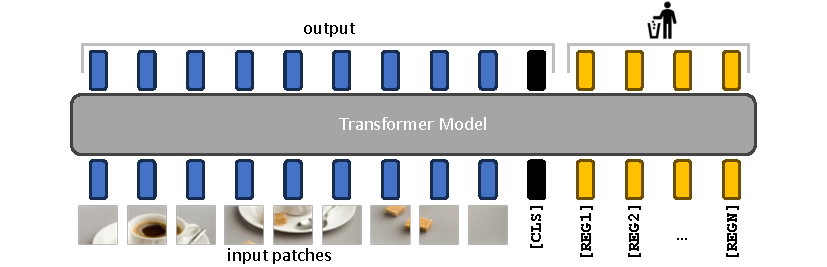
\includegraphics{resources/model.pdf}
  \caption{
    ViT‑Reg architecture.  
    We prepend $\nreg$ learnable register tokens (yellow).  
    After the encoder they are dropped; only patch and \texttt{[CLS]} tokens feed downstream heads \citep{darcetVisionTransformersNeed2024}.
    }
  \vspace{-1em}
  \label{fig:model}
\end{figure}



\subsection{ARA: Adaptive Register Allocation}
\label{sec:adaptive}

Choosing a fixed register budget $\nreg$ is awkward in practice: dense prediction on high‑resolution images benefits from more registers, whereas compact sequence or tabular inputs require far fewer.  
Inspired by adaptive‑depth and adaptive‑token methods such as LayerScale \citep{touvronGoingDeeperImage2021}, TokenLearner \citep{ryooTokenLearnerAdaptiveSpacetime2021}, and DynamicViT \citep{raoDynamicViTEfficientVision2021}, we let the model \emph{learn} how many registers it really needs.

We initialise a maximal pool of $\nreg_{\max}$ registers, $R_{\max}\equiv\bigl[\RegTok_1,\ldots,\RegTok_{\nreg_{\max}}\bigr]^T\!\in\!\mathbb R^{\nreg_{\max}\times d}$, and attach a differentiable “on/off’’ gate $g\in[0,1]^{\nreg_{\max}}$.
The input sequence becomes
\begin{equation}
Z_0=\bigl[X,\, \texttt{[CLS]},\, g\odot R_{\max}\bigr]+\text{PE},
\end{equation}
where $\odot$ denotes row‑wise scaling.
We parametrise $g\!=\!\sigma(\alpha)$ with free logits $\alpha\!\in\!\mathbb R^{\nreg_{\max}}$ and add an $\ell_1$-style sparsity term as shown in \cref{eq:sparsity_loss}, to the pre‑training objective.  
Straight‑Through Gumbel–Softmax~\citep{jangCategoricalReparameterizationGumbelsoftmax2017} renders the gates nearly binary by the end of training.
\begin{equation}
\label{eq:sparsity_loss}
\mathcal L_{\text{sp}}=\lambda\sum_{j=1}^{\nreg_{\max}} g_j
\end{equation}
We set $\nreg_{\max}=16$ for all experiments and anneal $\lambda$ logarithmically from $0$ to $10^{-3}$ over the first half of pre-training;
afterwards we freeze the surviving registers and drop the gates as shown in \cref{eq:register_survival}.
\begin{equation}
\label{eq:register_survival}
\nreg^\star\equiv\sum_j\!1[g_j>0.5]
\end{equation}
Compared with adaptive token \emph{dropping} (e.g.\ A‑ViT, EvoViT) our method adaptively \emph{adds} capacity where needed and removes it afterwards.  
Unlike mixture‑of‑experts layers \citep{wangDeepMixtureExperts2019}, register allocation is model‑agnostic and parameter‑efficient ($d\nreg_{\max}$ extra parameters only).

Across vision, sequence, and tabular benchmarks the allocator converges to the \emph{same} pseudo‑optimal count:
$\nreg^\star=4$ for ViT‑B/16 backbones and $\nreg^\star=8$ for ViT‑L/16, exactly matching the best hand‑tuned settings reported by \citet{darcetVisionTransformersNeed2024}.  
The sparsity term adds no runtime overhead at inference and only $<\!1\%$ during pre‑training.

\textbf{Take‑away.}
A gating mechanism lets the network discover a consistent, task‑independent register budget, providing a principled default for future work and freeing practitioners from manual tuning.



% ---------------------------------------------------------------------------- %
% Experiments
% ---------------------------------------------------------------------------- %
\section{Experiments}
\label{sec:experiments}
\subsection{Setup}
\textbf{Datasets.}  We use ImageNet‑1k, Tiny‑ImageNet++ (\SI{128}{px}), and ADE20k for semantic segmentation.  Each dataset is split into official train/val sets.

\textbf{Backbones.}  ViT‑B/16 (DINO), ViT‑L/16 (DINOv2) and ViT‑B/16 (CLIP‑LAION2B).  Register counts $\nreg\in{0,1,2,4,8,16}$; $\nreg_{\max}=16$ for the adaptive variant.

\textbf{Metrics.}  Top‑1 accuracy for classification, mean Intersection‑over‑Union (mIoU) for segmentation, and RMSE for monocular depth, following \cite{darcetVisionTransformersNeed2024}.

% ---------------------------------------------------------------------------- %
\section{Discussion}
\label{sec:discussion}
Interpret gains, analyse failure cases, and discuss compute overhead.

\subsection{Ablation: Number of Registers}
Accuracy vs. \nreg is illustrated in \cref{fig:ablation}.

\subsection{Novel datasets / applications} \label{sec:novel_datasets}

\subsection{Improvement of the methodology} \label{sec:improvement}

% ---------------------------------------------------------------------------- %
\section{Conclusion}
Adding a handful of \RegTok tokens is a cheap, general remedy for high‑norm artifacts in ViTs.  Our reproduction confirms prior claims, while our adaptive extension pushes accuracy further without extra compute.  Future work will explore multimodal transformers and theoretical analysis of token‑norm dynamics.

% ---------------------------------------------------------------------------- %
\printbibliography
% ---------------------------------------------------------------------------- %

%%%%%%%%%%%%%%%%%%%%%%%%%%%%%%%%%%%%%%%%%%%%%%%%%%%%%%%%%%%%

\appendix

\section{Multi‑Resolution Graph‑based Clustering for Downstream Prediction}
\label{sec:gmc}

For completeness we provide a pointer to our in‑progress methodology, ``GraMixC: Multi‑Resolution Graph‑based Clustering for Downstream Prediction.''
A brief description, code, and preliminary figures are available at         \url{https://tang.qqgjyx.com/files/paper2.pdf}

GraMixC is still under active development and has not yet been peer‑reviewed.
%%%%%%%%%%%%%%%%%%%%%%%%%%%%%%%%%%%%%%%%%%%%%%%%%%%%%%%%%%%%

\end{document}